\section{System Design}
\label{sec:design}
AgentWorkShop is designed for industrial tasks whose agents, production
contexts, interfaces, and process signals vary between deployments. A useful
framework must let these differences be configured without changing the
shared task runtime, while ensuring that a proposed operation is checked
against the active production context before it reaches a device. It must also
retain enough route-specific evidence to distinguish a returned command
receipt from a measured process response.

\subsection{Design Rationale and Requirements}
\label{sec:principles}
Five requirements---scene variability, harness variability, operation
authority, outcome observability, and extensibility---organize six design
rules (D1--D6). These are deployment constraints drawn from the target
workflows. D1 stores scene settings as versioned data;
D2 provides registered harness, tool, and driver interfaces; D3 separates
proposal from execution; D4 treats the tool catalog as discovery rather than
permission; D5 routes actuator writes through the common DCW admission point;
and D6 retains evidence by operation.

The requirements trace to implementation and evaluation as follows.
Scene variability maps to D1, scene blueprints, and context resolution;
harness variability and extensibility map to D2, the registered harness and
driver interfaces; operation authority maps to D3--D5, the shared dispatcher,
grants, bindings, and write admission; outcome observability maps to D6,
route-specific receipts, and observations. In the evaluation, R13 exercises
two scene-specific protocol and data paths; R20 exercises the configured
task-to-device path through one registered harness, synthetic approvals, and
route-specific records. These tests do not isolate profile or binding changes
under matched conditions, establish third-party extension or cross-harness
portability, or show target attainment in R20. Older scripted and regression
records are retained in the companion evidence package, but do not support
the current integration claims. AgentWorkShop supplies task and operation
services; agent strategy and independent process protection remain outside
this design.

\subsection{Layered Architecture}
\label{sec:layers}
\label{sec:arch}
Fig.~\ref{fig:arch} maps the reference implementation onto six bands and
their route-specific evidence records. The access band exposes command-line,
web, SDK, REST, MCP, and A2A entry surfaces. Task and chat routes enter the
collaboration band, which contains workspaces, channels, task queues, shared
memory, mailboxes, task templates, and harness adapters. A direct REST
tool-invocation route can call the shared operation dispatcher without
creating a task or invoking a harness; MCP also includes separate management
and task operations. The governance band projects an operation catalog and
checks each invocation. The context band assembles bound-line and active-run
information for prompt grounding, while operation handlers resolve the live
state relevant to their route. The service band provides acquisition, write
control, analysis, retrieval, and optional model services. The field-I/O band
resolves semantic nodes to built-in or plugin drivers for a plant or
simulator.

Each band has a distinct responsibility. Task/chat routes enter the task
runtime; direct operation routes enter the dispatcher; and both use shared
operation checks where applicable. A harness adapter supplies
agent-specific interaction on task paths, semantic nodes hide protocol
details from operations, and the driver registry provides the device-facing
extension point. Owning services retain task, command, observation, and
version records separately and link them to available actor and production
context. No single status conflates these outcomes.

\subsection{Cross-Module Execution Flow}
\label{sec:executionflow}
Fig.~\ref{fig:runtime} summarizes a task turn from entry through operation
execution, with route-specific evidence retained by owning services. The
runtime assembles prompt-time production context and a scoped tool catalog
before invoking a registered harness. This context is grounding information
refreshed on each agent turn, not a task-pinned transaction. For
each returned tool call, the shared dispatcher rechecks invocation scope
and channel policy; industrial operations also receive current grant and
binding checks before handler selection. The selected handler applies its
own route-specific guards, approval, revalidation, and device-I/O steps.
Command receipts and any later process observations remain distinct records.

For an industrial operation $u$ by agent $a$ in channel $c$, define the
shared dispatch condition as
\begin{equation}
\mathcal{A}(a,c,u)=S(a,c,u)\land P(c,u)\land G(a,u)\land B(a,u),
\label{eq:dispatch-contract}
\end{equation}
where $S$, $P$, $G$, and $B$ denote invocation scope, current channel policy,
runtime grant, and agent binding/resource ownership, as applicable to the
operation. The policy term includes
the applicable channel tool selection, profile, and duty-separation checks.
This condition is necessary for handler selection, not sufficient for
actuation: the selected route applies its own guards and approval, then
rechecks authority and applicable limits before dispatch.

Fig.~\ref{fig:execution} gives pseudocode for these cross-module contracts;
it is a reference flow rather than one literal orchestrator function.
Route-specific timing, approval, and evidence rules are detailed in
Section~\ref{sec:modules}.

\begin{figure*}[!t]
\centering
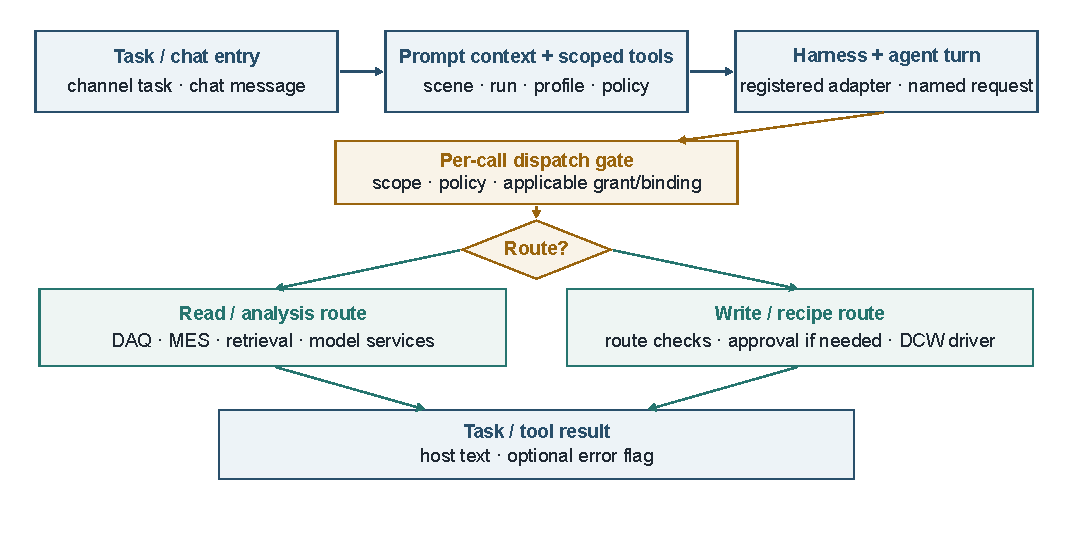
\includegraphics[width=\textwidth]{resources/fig-runtime-2026-9pt.pdf}
\caption{Cross-module task execution in AgentWorkShop. The task path assembles
a channel-scoped tool catalog and per-turn prompt context. Each returned call
is rechecked for scope and policy; the handler resolves applicable live state,
including grant, binding, and active-run checks on recipe operations. The
shared tool result contains host text and an optional error flag; route
records remain with owning services. The prompt-time context is not passed as
a transactional authorization token. Dispatch-gate errors return before
handler execution, whereas route-specific handlers may read state before
refusing a write. Durable denial auditing is selective. Receipts and later
observations remain distinct.}
\label{fig:runtime}
\end{figure*}

\begin{figure}[!t]
\centering
\begin{algorithmic}[1]
\Require task $q$, channel $c$, bound agent $a$
\Ensure task result; any retained evidence remains with its owning service
\State $x_t \gets \Call{ResolvePromptContext}{c,q}$
\State $T \gets \Call{FilterToolCatalog}{a,c}$
\State $m \gets \Call{RetrieveMemory}{q}$
\State $p \gets \Call{AssemblePrompt}{q,x_t,m}$
\State $h \gets \Call{InvokeRegisteredHarness}{a,p,T}$
\ForAll{tool request $u$ returned by $h$}
  \State $g \gets \Call{CheckScopeAndChannelPolicy}{a,c,u}$
  \If{\textbf{not} $g$}
    \State \Call{ReturnToolError}{h,u}; \textbf{continue}
  \EndIf
  \If{$u$ is an industrial operation}
    \State $v \gets \Call{CheckGrantBindingOwnership}{a,u}$
    \If{\textbf{not} $v$}
      \State \Call{ReturnToolError}{h,u}; \textbf{continue}
    \EndIf
  \EndIf
  \State $k \gets \Call{SelectHandler}{u}$
  \State $r \gets \Call{ExecuteRouteHandler}{k,a,c,u}$
  \Comment{handler resolves live state and may persist route-specific records}
  \State \Call{ReturnDeclaredToolResult}{h,r}
\EndFor
\State \Return task state and tool results
\end{algorithmic}
\caption{Reference pseudocode for cross-module execution in AgentWorkShop.
Evidence persistence is route-specific and remains with the owning service;
the shared tool result does not carry a generic evidence envelope.}
\label{fig:execution}
\end{figure}
